

\thesischapter{Formalising the European Rail Traffic Management System Using Hybrid Automata}
The ERTMS system will be central to many train control systems in the future and ensuring that it is safe is of paramount importance. It poses a particular challenge due to the fact that the system is specified at a high level with each individual country having its own particular implementation. One aspect that is particularly problematic and loosely specified is the interface between the existing interlocking and the RBC as both of these systems have a role to play in ensuring safety. In the following chapter we shall look at formalising the ERTMS system whilst capturing the behaviour of this critical interface between the two systems. 


\section{Hybrid Automata}

One formalism which we can use to reason about systems such as ERTMS is hybrid automata \cite{TH96}. We shall give a theoretical overview of Hybrid Automata before formalising ERTMS as three Hybrid automata composed in parallel. A hybrid automaton has discrete states called control modes and transitions between these modes called control switches. These control switches are triggered by either some condition on variables or by some event occurring. These events can either occur in some other automaton or they can be fired by an automaton due to some condition being met. The continuous transitions of the automaton are described by dotted variables\footnote{The dotted variables represent the rate of change of a given variable over time $\dot{y} = \frac{dy}{dt}$. This notation was introduced by Newton \cite{CF28}.} and occur continually over time.

\medskip
\begin{mydef}[Hybrid Automaton: Syntax]
The syntax of a hybrid automaton $H$ comprises of the following:
\begin{description}
\item[Variables] A finite set $X = \{x_1, \ldots x_n \}$ of variables which range over the real numbers. The cardinality of $|X|$ is called the \emph{dimension} of $H$. The variable set has a corresponding dotted variable set $\dot{X} = \{\dot{x}_1, \ldots \dot{x}_n \}$ which represents the continuous changes of variables and a primed variable set $X' = \{x'_1, \ldots , x'_n \}$ that represents  values at the conclusion of a discrete change.

\item[Control graph] A finite directed multigraph $(V,E)$ consisting of a set of vertices which we shall refer to as \emph{control modes} and a set of edges $E$ which we shall refer to as \emph{control switches}.

\item[Initial, invariant and flow conditions] Three functions \emph{init},\emph{inv} and \emph{flow} that label each control mode $v \in V$ with three predicates such that for all $v \in V$, $\freevar{init(v)} \subseteq X$, $\freevar{inv(v)} \subseteq \dot{X}$ and $\freevar{flow(v)} \subseteq X \cup \dot{X}$. 


\item[Jump Conditions] A function \emph{jump} that labels each edge $e \in E$ with a predicate such that $\freevar{jump(e)} \subseteq X \cup X' $.

\item[Events] A finite set $\Sigma$ of \emph{events}, at least one of which is assigned to  each control switch by a labelling function $event: E \to \Sigma$.

\end{description}
Where $\freevar{P}$ is the set of free variables in the predicate $P$.
\end{mydef}
\medskip


\medskip
\section{Pentagon Example}

\medskip
The following is a simple example railway we shall use for the purposes of demonstrating our verification approach.  It contains 5 track segments connected to form a pentagon with two trains. This captures most of the behaviours found in a larger more complicated railway as the trains and control systems view any piece of track as a set of track segments joined together to form a route.

\begin{figure} [h!]

\begin{center}
\begin{tikzpicture}[node distance = 3cm]


\node (A) [draw,regular polygon, regular polygon sides=5, minimum size=6 cm,outer sep=0pt] {};
\foreach \n in {1,...,5} {

    \pgfmathtruncatemacro{\value}{(\n - 1) * 50};
    \node at (A.corner \n) [anchor=360/5*(\n-1)+270] {D = \value};
    \node at (A.side \n) [anchor = 360/5 *(\n-1) +270] {$t_{\n}$};
}

\node (B) [draw, rectangle, rotate = 36] at (-1.9,2.6) {Train A};
\node (C) [draw, rectangle, rotate =72] at (3,-1) {Train B};

\end{tikzpicture} 
\end{center}

\label{fig:trackplan2}
 \caption{Pentagon Example}
\end{figure}

\begin{comment}



\def\r{3} 
\def\sone{ \sin 32}
\def\stwo{\sin 72}
\def\cone{\cos 32}
\def\ctwo{\cos 72}
\coordinate(top) at (0,\r);
\coordinate(topleft) at ({ \r * -cos (36)},{ \r * -sin (36)});
\coordinate(topright) at ({ \r * cos (72)}, { \r * -sin (72)});
\coordinate(botleft) at ({ \r * - cos (36)},{ \r * sin (36)});
\coordinate(botright) at ({\r * sin (72)},{\r * cos (72)});

\tikzstyle{box1}=[circle, draw, text width = 2cm, font=\scriptsize]
\tikzstyle{box3}=[rectangle, draw, text width = 2cm, font=\scriptsize]
\tikzstyle{arrow}=[->, thick]
\tikzstyle{biarrow}=[<->,very thick,shorten >=7pt,shorten <=7pt]


\node (A) [font = \scriptsize]  at (topleft)                  {D =150 };

\node (B) [font = \scriptsize]    at (botleft)          {D = 0};

\node (C)[font = \scriptsize] at (top)  { D = 100
						};

\node (D)[font = \scriptsize] at (botright)  { D = 50
						};

\node (E) [font = \scriptsize] at (topright) {D = 200};

\draw [arrow] (D) -- node[right] {$t_1$} (E);
\draw [arrow] (A) -- node[below = 10pt] {$t_4$} (B);
\draw [arrow] (B) --  node[above = 10pt] {$t_2$} (C);
\draw [arrow] (C) -- node [left] {$t_3$} (D);
\end{comment}
We have modelled the ERTMS system controlling the pentagon example (see fig \ref{fig:trackplan2}) using several hybrid automata. In this example the value $D(t)$ represents the distance from the start point at time $t$. 
It contains 2 trains $A$ and $B$ and 5 track circuits $l_0, \ldots , l_4$. The track is uni-directional allowing trains to travel from $0 - 249$. 
\medskip




We start by defining a hybrid automaton for the interlocking consisting of 2 states representing whether a request have been made or not, 5 boolean variables representing whether a track segment is occupied or not and a variable $ReqID$ which stores the last requested track segment. When a request for a track segment is made that track segment is stored and then if the track freedom condition is met then a request is granted, otherwise it is denied. The event $l_x.l_{x+1}$ captures the movement of a train from one track segment to the next in both the interlocking automaton and the train automaton.
\medskip
\begin{mydef}[Interlocking Hybrid Automaton]
We define a hybrid automaton $H_{IL}$ as follows:
\begin{description}
\item[Variables] The state of the interlocking automaton consists of five boolean variables  $\underbrace{l_0, \ldots , l_4}_\text{Occupied/Free}$ and a variable $ReqID$ ranging over $\{0 , \ldots , 4 \}$.

\item[Control Graph] The control graph of the interlocking automaton consists of two control modes $\{Response, Idle \}$ with four control switches connecting them; $Response \to Idle$, $Idle \to Response$, $Response \to Response$, $Idle \to Idle$.

\item[Initial, invariant and flow conditions] \hspace*{0mm}
	\begin{itemize}
	\item $init(Idle) := [l_0 = Free, l_1 = Free, l_2 = Free, l_3 = Free, l_4 = Free]$.

	\end{itemize}

\item[Jump Conditions] \hspace*{0mm}

	\begin{itemize}
	\item $jump(Idle \to Response) :=  Req.z , ReqId' = z$

	
	\item $jump(Response \to Idle) := \mathbf{if} \ (l_{ReqId} = Free \wedge l_{ReqId +1 \, mod \, 5} = Free)$ \\
             \hspace{\fill} $\mathbf{then} \ Grant. ReqId \ \mathbf{else} \ Deny.ReqId$ 

	\item $jump(Idle \to Idle) := l_x. l_{x+1} , [l_x' = Free, l_{x+1}' = Occupied]$

	\item $jump(Response \to Response) := l_x. l_{x+1} , [l_x' = Free, l_{x+1}' = Occupied]$


	\end{itemize}

\item[Events] \hspace*{0mm}
\begin{itemize}
	\item $event (Idle \to Response) := Req.z$
	\item $event(Response \to Idle) :={Grant.z,Deny.z}$
	\item $event(Idle \to Idle) := l_x.l_{x+1}$
	\item $event(Response \to Response) := l_x.l_{x+1}$	
\end{itemize}

\end{description}
\end{mydef} 
\medskip
\FloatBarrier
\begin{figure} [H]

\begin{center}
\begin{tikzpicture}[scale = 0.60]

\tikzstyle{box1}=[circle, draw, text width =3cm]
\tikzstyle{box3}=[rectangle, draw, text width = 2cm, font=\scriptsize]
\tikzstyle{arrow}=[->,shorten >=7pt,shorten <= 7pt]
\tikzstyle{biarrow}=[<->,very thick,shorten >=7pt,shorten <=7pt]



\node (B) [box1]    at (7.5,0)          {\begin{center} \textbf{Idle} \\ \end{center}

};

\node (C)[box1] at (0, 7.5)  { \begin{center} \textbf{Response}\\ \end{center}                                               
						};


\draw [arrow] (B)  .. controls +(-1.5 cm,  2.75 cm) and +(4.5cm,  -2.5cm ) .. node [right, text width=4cm] {Req.z} (C);
\draw [arrow] (C) .. controls +(1cm,  -3cm) and +(-2.75cm, 1 cm ) ..   node [left = 3 cm, below, text width = 6cm] {$Grant.z \  \mathbf{if} \ t_{ReqId} = \ free $\\$ \mathbf{else} \ Deny.z \ Otherwise$} (B);


\end{tikzpicture} 
\end{center}

\label{fig:ILAuton}
\caption{Interlocking Automaton}
\end{figure}
The behaviour of the train is based on two of Newtons laws of motion $v = u +at$ and  $v^2 = u^2 +2as$
,where s = displacement,u = initial velocity, v = final velocity, a = acceleration and t = time. In order to model the behaviour of trains we make use of two functions, one to compute the braking distance at the current speed and the other to compute the distance from the train to the end of the movement authority. When the values computed by these two functions become equal the train should begin to brake in order to stop at the end of the movement authority. The simplest way to model deceleration would be to assume that the trains speed decreases at $-1$ unit of distance per unit of time. The second equation of motion  is used to caluate the breaking distance with $u = 0$ and $a = 1$ it can be rewritten to allow for the calculation of the breaking distance.
\medskip

\newcommand{\BD}[1]{\mathrm{BD}(#1)}
\begin{mydef}[Breaking Distance]
We define the breaking distance for a train in terms of its speed as follows:

$$\BD{S} = \frac{S^2}{2} $$

\end{mydef}
\medskip
Since we are working with a loop in the track the distance to the movement authority is calculated modulo the length of the track. 
\medskip
\newcommand{\DMA}[2]{\mathrm{DMA}(#1,#2)}
]\begin{mydef}[Distance to Movement Authority]

The distance to the movement authority $\mathrm{DMA}$ is calulated from the distance and movement authority as followings:
\begin{align*}
\DMA{D(t), MA} & = MA \Monus D(t) \quad \mathbf{if} \ D(t) \leq MA \\
                         & = 50 \Monus D(t) + MA \quad \mathbf{otherwise}
\end{align*}



\end{mydef}

The Train hybrid automaton has $4$ control modes namely Braking (Auth), Full Allowed Speed, Accelerating and Stopped and has $5$ variables namely $Maxspeed$,$D(t)$ (Position),  $Speed$, $\dot{Speed}$ and $EoA$. We have that $ BD(Speed) \leq DMA(D(t), EoA)$ is an invariant of the stopped mode and $D(t) \leq EoA$ is an invariant of all other control modes.
We define a mode jump with the event $l_x.l_{x+1}$ which is triggered by the condition $D \,  mod \, 50 = 0$ in the modes $Full Speed$, $Accelerating$ and $Brake$. 
   We compose both the automata for both the interlocking and the hybrid $H_{IL} || H_{T}$. It is possible for a new MA $EoA'$ with $EoA < EoA'$ to be received in the $Braking$ and $Stopped$ states.  This is triggered by the event MA.x.y if $x = TrainID$ then $y$ becomes the new movement authority. The movement event MA.Req.x is used by a train automaton request a movement authority for train x from the RBC automaton. Secondly we define a hybrid automaton $H_{T}$ which models an individual train. 
\medskip
\begin{mydef}[Train Automaton]

We define a hybrid automaton $H_{T}$ as follows:
\begin{description}
\item[Variables] The state of the interlocking automaton consists of $\underbrace{D(t), EoA}_\text{0, \ldots , 249}$, \newline $\underbrace{Speed, \dot{Speed}, MaxSpeed, TrainID}_{\mathbb{N}}$. The variable D(t) is computed modulo 250 from Speed.

\item[Control Graph] The control graph of the interlocking automaton consists of four control modes $\{Stop (EoA), \, Braking, \, Accelerating, \, Full \, Allowed \, Speed \}$.

\item[Initial, invariant and flow conditions] \hspace*{0mm}
	\begin{itemize}
	\item $init(Stopped) :=   BD(S) \leq DMA(D(t),EoA)  $.

	\item $inv(Full Allowed Speed) :=   \dot{Speed} = 0 \wedge BD(S) \leq DMA(D(t),EoA)$ 

	\item $inv(Braking)  := inv(Accelerating) := BD(S) \leq DMA(D(t),EoA)$

	
	\item $inv(Stop (EoA)) := Speed = 0$ 
             
	\item $flow(Accelerating):= \dot{Speed} = 1$ 
	
	\item $flow(Braking) := \dot{Speed} = -1$
 
	\end{itemize}

\item[Jump Conditions] \hspace*{0mm}

	\begin{itemize}
	\item $jump(Full Allowed Speed \to Full Allowed Speed) := l_{D(t) \, div \, 50}.l_{(D(t) \, div \, 50) +1} \wedge D(t) \, mod \, 50 = 0$
\item $jump(Braking \to Braking) = l_{D(t) \, div \, 500}.l_{(D(t) \, div \, 50) +1} \wedge D(t) \, mod \, 50 = 0$
\item $jump(Accelerating \to Accelerating) = l_{D(t) \, div \, 500}.l_{(D(t) \, div \, 50) +1} \wedge D(t) \, mod \, 50 = 0$

	\item  $jump(Braking \to Accelerating) := jump(Stop (EoA) \to Accelerating) := MA.x.y\\ \textbf{if} x = TrainID \\ \textbf{then} MA := y$ 
	

	\item $jump(Full Allowed Speed \to Braking) :=jump(Accelerating \to Braking) := DMA(D(t),EoA) = BD(Speed), MA.Req.TrainID$


	\item $jump(Accelerating \to Full Allowed Speed)$ := Speed = MaxSpeed
	
	\item $jump(Braking \to Stop (EoA)) := Speed = 0$

	\end{itemize}

\item[Events] \hspace*{0mm}
\begin{itemize}
	\item $event (Stop (EoA) \to Accelerating) := MA.TrainID.y$
	\item $event (Braking \to Accelerating) := MA.TrainID.y$
	\item $event(Full Allowed Speed \to Full Allowed Speed) := l_{D(t) \, div \, 50}.l_{(D(t) \, div \, 50) +1} \wedge D(t) \, mod \, 50 = 0$
\item $event(Braking \to Braking) = l_{D(t) \, div \, 50}.l_{(D(t) \, div \, 50) +1} \wedge D(t) \, mod \, 50 = 0$
\item $event(Accelerating \to Accelerating) = l_{D(t) \, div \, 50}.l_{(D(t) \, div \, 50) +1} \wedge D(t) \, mod \, 50 = 0$

	\item $event(Accelerating \to Braking) = MA.Req.TrainID$
	\item $event(Full Allowed Speed \to Braking) = MA.Req.TrainID$
\end{itemize}

\end{description}
\end{mydef}

\FloatBarrier
\begin{figure} [H]

\begin{center}
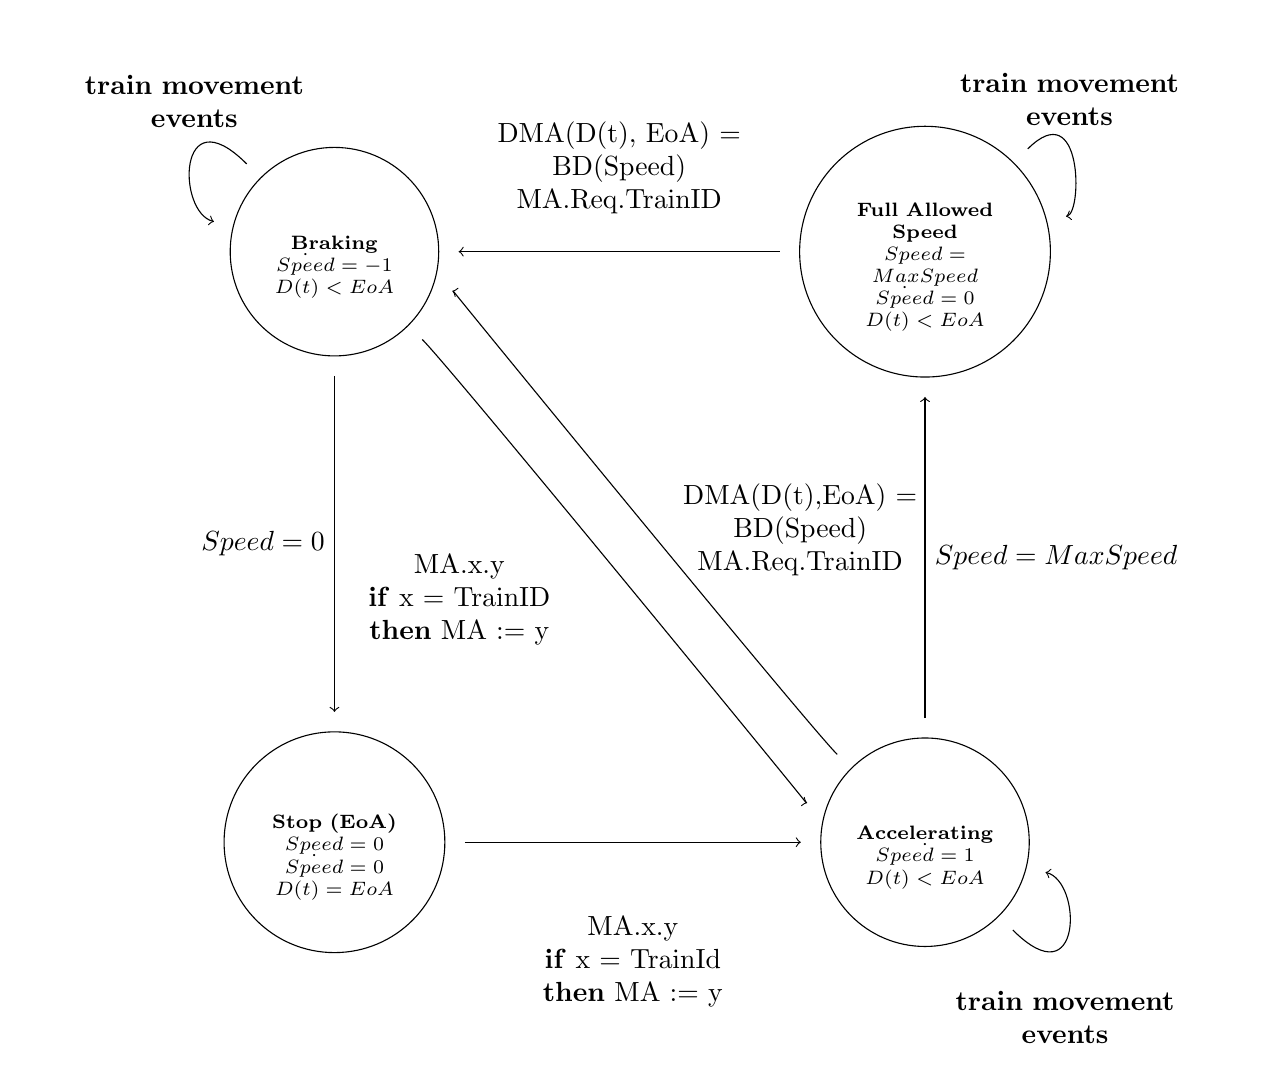
\begin{tikzpicture}[node distance = 2cm]

\tikzstyle{box1}=[circle, draw, text width = 2cm, font=\scriptsize]
\tikzstyle{box3}=[rectangle, draw, text width = 2cm, font=\scriptsize]
\tikzstyle{arrow}=[->,shorten >=7pt,shorten <= 7pt]
\tikzstyle{biarrow}=[<->,very thick,shorten >=7pt,shorten <=7pt]


\node (A) [box1]  at (0,0)                  {\begin{center} \textbf{Stop (EoA)} \\
							$Speed = 0$
                                                        $\dot{Speed} = 0$
							$D(t) = EoA$  \end{center}

                                            };

\node (B) [box1]    at (7.5,0)          {\begin{center} \textbf{Accelerating} \\
       $\dot{Speed = 1}$
       $D(t) < EoA$  \end{center}

};

\node (C)[box1] at (0, 7.5)  { \begin{center} \textbf{Braking}\\
					                   $\dot{Speed} = -1$ 
						           $D(t) < EoA$\end{center}
                                               
						};

\node (D)[box1] at (7.5, 7.5)  { \begin{center} \textbf{Full Allowed Speed }\\
					                   $Speed = MaxSpeed$
                                                            $\dot{Speed} = 0$
							    $D(t) < EoA$
                                                            \end{center}
                                               
						};


\draw [arrow] (B) -- node[right] {$Speed = MaxSpeed$} (D);
\draw [arrow] (A) -- node[below = 10pt, text width = 4cm] {\begin{center}MA.x.y\\ \textbf{if} x = TrainId\\ \textbf{then} MA := y\end{center} } (B);
\draw [arrow] (D) --  node[above = 10pt,text width=4cm] {\begin{center}DMA(D(t), EoA) =\\ BD(Speed)\\MA.Req.TrainID \end{center}} (C);
\draw [arrow] (C) -- node [left] {$Speed = 0$} (A);
\draw [arrow] (B)  .. controls +(-1.5cm,  1.5 cm) and +(1.5cm,  -0.5 cm ) .. node [right,text width=4cm] { \begin{center}DMA(D(t),EoA) =\\
    BD(Speed)\\MA.Req.TrainID \end{center}} (C);
\draw [arrow] (C) .. controls +(1.5cm,  -1.5cm) and +(-1.5cm, 0.5 cm ) ..   node [left,text width = 4cm] {\begin{center}MA.x.y\\ \textbf{if} x = TrainID \\ \textbf{then} MA := y\end{center} } (B);
\draw [arrow] (C) .. controls +(-2cm,  2cm) and +(-2cm, 0.5 cm ) ..   node [above = 10pt, text width = 4cm] {\begin{center}\textbf{train movement events} \end{center}} (C);
\draw [arrow] (D) .. controls +(2cm,  2cm) and +(2cm, 0.5 cm ) ..   node [above = 10pt, text width = 4cm] {\begin{center} \textbf{train movement events} \end{center}} (D);
\draw [arrow] (B) .. controls +(2cm,  -2cm) and +(2cm, -0.5 cm ) ..   node [below = 6pt, text width = 4cm] {\begin{center}\textbf{train movement events} \end{center}} (B);

\end{tikzpicture} 
\end{center}

\label{fig:TrainAuto}
\caption{Train Automaton}


\end{figure}




\begin{comment}



\begin{figure} [H]

\begin{center}
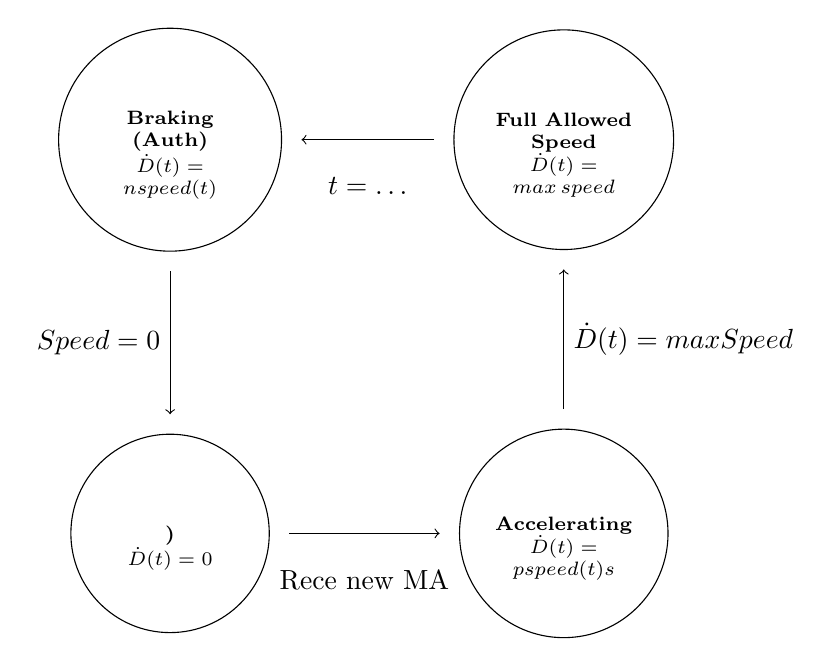
\begin{tikzpicture}[node distance = 3cm]

\tikzstyle{box1}=[circle, draw, text width = 2cm, font=\scriptsize]
\tikzstyle{box3}=[rectangle, draw, text width = 2cm, font=\scriptsize]
\tikzstyle{arrow}=[->,shorten >=7pt,shorten <=7pt]
\tikzstyle{biarrow}=[<->,very thick,shorten >=7pt,shorten <=7pt]


\node (A) [box1]  at (0,0)                  {\begin{center} \textbf{)} \\
							$\dot{D}(t) = 0$  \end{center}

                                            };

\node (B) [box1]    at (5,0)          {\begin{center} \textbf{Accelerating} \\
       $\dot{D}(t) = pspeed(t)s$  \end{center}

};

\node (C)[box1] at (0, 5)  { \begin{center} \textbf{Braking (Auth)}\\
					                   $\dot{D}(t) = nspeed(t)$ \end{center}
                                               
						};

\node (D)[box1] at (5, 5)  { \begin{center} \textbf{Full Allowed Speed }\\
					                   $\dot{D}(t) = max\, speed$ \end{center}
                                               
						};


\draw [arrow] (B) -- node[right] {$\dot{D}(t) = max Speed$} (D);
\draw [arrow] (A) -- node[below = 10pt] {Rece new MA} (B);
\draw [arrow] (D) --  node[below = 10pt] {$t = \ldots$} (C);
\draw [arrow] (C) -- node [left] {$Speed = 0$} (A);


\end{tikzpicture} 
\end{center}

\label{fig:TrainAuton}
\caption{Train Automaton}
\end{figure}
\end{comment}

\medskip
Similarly to the train automaton the RBC automaton also has four control modes namely Granted, Idle, Wait and Ready to Request. Initially the system is in an idle state where the system waits until it receives a movement authority request MA.Req.x. When the train receives such a movement authority request the LastTrain variable is assigned to be x and the system moves to the Ready to Request state.  From this state the train sends a request for the next track segment of the LastTrain.
\medskip

\begin{mydef}[Radio Block Controller Hybrid Automaton]

We define a hybrid automaton $H_{RBC}$ as follows:
\begin{description}
\item[Variables] The state of the radio block controller automaton consists of $\underbrace{MA_1, Pos_1, MA_2, Pos_2}_\text{0, \ldots , 2499}$, \newline $\underbrace{LastTrain}_{\mathbb{N}}$.

\item[Control Graph] The control graph of the radio block controller automaton consists of four control modes $\{Idle, \, Ready \, to \, Request, \, Wait, \, Granted \}$.

\item[Initial, invariant and flow conditions] \hspace*{0mm}
	\begin{itemize}
	\item $init(Idle) :=   \ldots $

	\end{itemize}

\item[Jump Conditions] \hspace*{0mm}

	\begin{itemize}
	\item $jump(Ready to Request \to Ready to Request) := Train.x.Pos.y \wedge MA.x = y$
	\item $jump(Wait \to Wait) := Train.x.Pos.y \wedge MA.x = y$
	\item $jump(Granted \to Granted) := Train.x.Pos.y \wedge MA.x = y$
	\item $jump(Idle \to Idle) := Train.x.Pos.y \wedge MA.x = y$
	\item $jump(Idle \to Ready to Request) := MA.Req.x \wedge LastTrain = x$
	\item $jump(Ready to Request \to Wait) := Req.NextTrack(TrackSeg(Pos.LastTrain))$
	\item $jump(Wait \to Ready to Request) := Deny.LastTrain$
	\item $jump(Wait \to Granted) := Grant.LastTrain$
	\item $jump(Granted \to Idle) := MA.x.EndOf(z)$



	\end{itemize}

\item[Events] \hspace*{0mm}
\begin{itemize}
\item $jump(Ready to Request \to Ready to Request) := Train.x.Pos.y$
	\item $jump(Wait \to Wait) := Train.x.Pos.y$
	\item $jump(Granted \to Granted) := Train.x.Pos.y $
         \item $jump(Idle \to Idle) := Train.x.Pos.y$
	\item $jump(Idle \to Ready to Request) := MA.Req.x $
	\item $jump(Ready to Request \to Wait) := Req.NextTrack(Pos.LastTrain)$
	\item $jump(Wait \to Ready to Request) := Deny.x$
	\item $jump(Wait \to Granted) := Grant.x$
	\item $jump(Granted \to Idle) := MA.LastTrain.EndOf(NextTrack(Pos.LastTrain)))$
\end{itemize}

\end{description}

\end{mydef}

\FloatBarrier

\begin{figure} [H]

\begin{center}
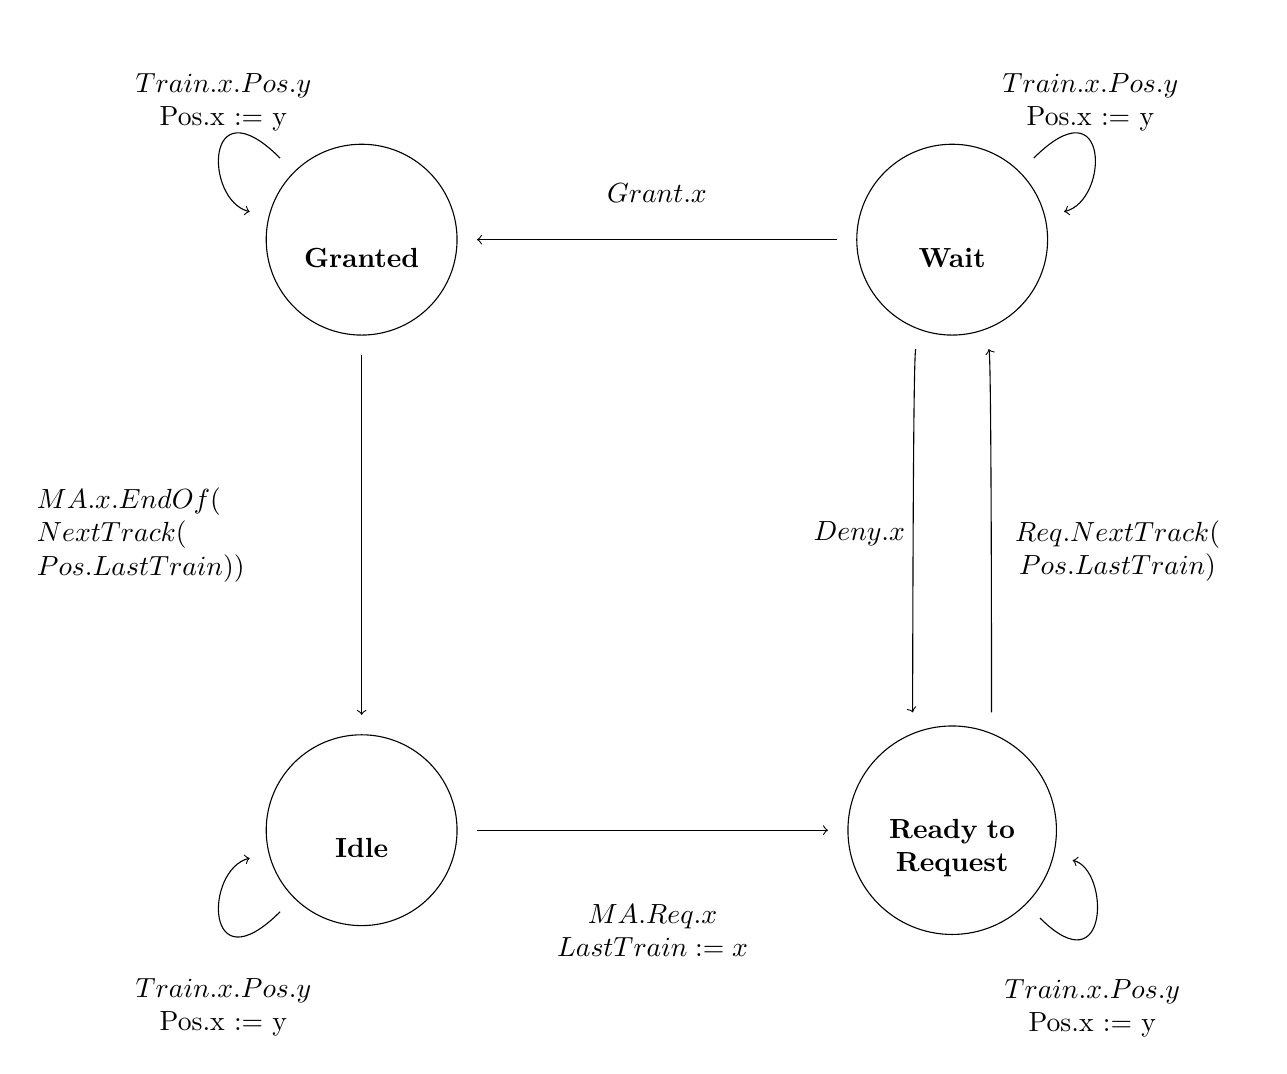
\begin{tikzpicture}[node distance = 1cm]

\tikzstyle{box1}=[circle, draw, text width = 2cm ]
\tikzstyle{box3}=[rectangle, draw, text width = 2cm, font=\scriptsize]
\tikzstyle{arrow}=[->,shorten >=7pt,shorten <= 7pt]
\tikzstyle{biarrow}=[<->,very thick,shorten >=7pt,shorten <=7pt]


\node (A) [box1]  at (0,0)                  {\begin{center} \textbf{Idle} \\
\end{center}};

\node (B) [box1]    at (7.5,0)          {\begin{center} \textbf{Ready to Request} \\
 \end{center}

};

\node (C)[box1] at (0, 7.5)  { \begin{center} \textbf{Granted}\\
					                \end{center}
                                               
						};

\node (D)[box1] at (7.5, 7.5)  { \begin{center} \textbf{Wait}\\
				
                                                            \end{center}
                                               
						};


\draw [arrow] (B)  .. controls +(0.5cm,  1.5 cm) and +(0.5cm,  -1.5 cm ) .. node[right, text width = 3cm] {\begin{center}$Req.NextTrack($ \\ $Pos.LastTrain)$ \end{center}} (D);
\draw [arrow] (D) .. controls +(-0.5cm,  -1.5cm) and +(-0.5cm, 1.5 cm ) ..   node [left] {$Deny.x$} (B);
\draw [arrow] (A) -- node[below = 10pt, text width = 4cm] {\begin{center}$MA.Req.x$ \\ $LastTrain := x$\end{center}} (B);
\draw [arrow] (D) --  node[above = 10pt,text width=4cm] {\begin{center}$Grant.x$\end{center}} (C);
\draw [arrow] (C) -- node [left, text width = 4cm] {$MA.x.EndOf($ \\ $NextTrack($ \\ $Pos.LastTrain))$} (A);

\draw [arrow] (C) .. controls +(-2cm,  2cm) and +(-2cm, 0.5 cm ) ..   node [above = 5pt, text width = 4cm] {\begin{center}$Train.x.Pos.y$\\ Pos.x := y\end{center}} (C);
\draw [arrow] (D) .. controls +(2cm,  2cm) and +(2cm, 0.5 cm ) ..   node [above = 5pt, text width = 4cm] {\begin{center}$Train.x.Pos.y$\\ Pos.x := y\end{center}} (D);
\draw [arrow] (B) .. controls +(2cm,  -2cm) and +(2cm, -0.5 cm ) ..   node [below = 6pt, text width = 4cm] {\begin{center}$Train.x.Pos.y$\\ Pos.x := y\end{center}} (B);
\draw [arrow] (A) .. controls +(-2cm,  -2cm) and +(-2cm, -0.5 cm ) ..   node [below = 6pt, text width = 4cm] {\begin{center}$Train.x.Pos.y$\\ Pos.x := y\end{center}} (A);


\end{tikzpicture} 
\end{center}

\label{fig:RBCAuton}
\caption{Radio Block Processor Automaton}
\end{figure}


Safety conditions for the combined system can be separated into discrete and continuous parts.  If we want to specify a safety condition which states that it is not possible for two trains to collide in our current system this could have the following components. 

the continuous part would state that any movement authority issued by the radio block processor would respect the interlockings separation policy. \textbf{(Note: I should up date this part at some point. In the current Maude implementation the interlocking will grant a track segment if it is not occupied)} The discrete part would basically state that there is at least two free track circuits in-between each train.

\section{Semantics of Hybrid Automata}

The semantics of the hybrid automaton are described using labelled transitions systems. These transition systems allow us to model the behaviour of a system with a possibly infinite number of discrete labelled states. 
\medskip
\begin{mydef}[Labelled Transition System]
We define a \emph{labelled transition system} $LTS = (S,S_0,T,L)$ as follows:
\begin{itemize}

\item $S$ is a possibly infinite set of states

\item $S_0$ is a set of initial states $S_0 \subseteq S$

\item $L$ is a set of \emph{labels}

\item $T$ is a binary relation $\xrightarrow{a}$ over the state space $S$.

\end{itemize}
\end{mydef}
\medskip
When defining the semantics of a hybrid automata we need to be able to speak about parts of the state space.  We define a \emph{region} as being a subset of the state space $R \subseteq S$.  This enables us to define, for example, a continous region for an initial state of a system rather than a discrete state. The semantics of hybrid automata are defined in terms of a timed transition system ...


\medskip
\begin{mydef}[Transition Semantics of Hybrid Automata]
We define the semantics of a hybrid automaton $H$ in terms of a \emph{timed transition system} $LTS^t_H = (S,S_0,L,T)$ as follows:


\begin{itemize}
 
\item The state space $S$ of the timed transition system is defined as, $S, S_0 \subseteq V \times R^n$. A state is in the state space $(v,x) \in S_0$ iff the closed predicate $inv(v)[X := x]$ holds. In addition to the previous condition a state is in the initial state space $(v,x) \in S_0$ iff the closed predicate $init(v)[X := x]]$ holds. We call a subset of the state space $S$ a \emph{H-region}.


\item $L = \Sigma \cup R {\geq 0}$

\item For all events $\sigma \in \Sigma$ such that there exists a control switch $e \in E$, define $(v,x) \xrightarrow{\sigma} (v',x')$ iif the following conditions are satisfied:
\begin{enumerate}
\item the source and target of $e$ are $v$ and $v'$ respectively. 
\item the closed predicate $jump(e)[X, X' := x,x']$ holds.
\item $event(e) = \sigma$.
\end{enumerate}

\item We define a transition $(v,x) \xrightarrow{\delta} (v,x')$ for all non-negative reals $\delta \in R_{\geq 0}$ iff there exists a differentiable function $f: [0, \delta] \to R^n$ such that the following holds:
\begin{enumerate}
\item The functions first derivative is $\dot{f} :(0,\delta) \to R^n$
\item $f(0) = x$
\item $\forall \epsilon \in (0,\delta)$ both of the predicates $inv(v)[X := f(\epsilon)]$ and $flow(v)[X,\dot{X} := f(\epsilon),\dot{f}(\epsilon)]$ hold.
\end{enumerate}
We call the function f the \emph{witness} of the transition $(v,x) \to (v, x')$

\end{itemize}


\end{mydef}
\medskip
\begin{mydef}[$q_0$-rooted and initialised trajectories]
Given a labelled transition system $LTS = (S,T,S_0,L)$ and a state $s \in S$. We define a $q_0$-\emph{rooted} \emph{trajectory} as a finite or infinite sequence of pairs $\langle a_i, q_i \rangle_{i \geq 1}$ of labels $a_1 \in L$ and states $q_i \in S$  such that $q_{i-1} \xrightarrow{a_i} q_{i} \in T$ for all $i \geq 1$. If $q_0 \in S_0$ then the sequence of pairs $\langle a_i, q_i \rangle_{I \geq 1}$ is an \emph{initialized trajectory}. 
\end{mydef}
\medskip
\begin{mydef}
We define a live transition system (LTS,A) to consist of a labelled transition system $LTS$ and a set $A$ of infinite initialised trajectories of $LTS$. If for all of the finite initialised trajectories of $LTS$ there exists an infinite trajectory in $A$ such that the finite trajectory is a prefix of the infinite one then we call $A$ \emph{machine-closed}. We define a \emph{trace} $\langle a_i \rangle_{i \geq 1}$ of (LTS,A) to consist of the labels from the either a finite initialised trajectory of $LTS$ or a trajectory in $A$.
\end{mydef}
\medskip

\begin{mydef}[Trace semantics of hybrid automata]
All transitions of a timed transition system $S^t_H$ have an associated \emph{duration} $\delta \in R_{\geq 0}$. Every event $\sigma \in \Sigma$ the transition $q \xrightarrow{\sigma} q'$ has a duration of 0. For all transition $q \xrightarrow{\delta} q'$ where $\delta \in R_{\geq 0}$ the duration is $\delta$.  We define an infinite trajectory $\langle a_i, q_i \rangle_{i \geq 1}$ of a transition system $S^t_H$ to be \emph{divergent} if the sum of the transitions $\Sigma_{i \geq 1} \delta$ is \emph{divergent}.
 \end{mydef}

\section{Automaton Validation}


We will now give a proof by induction that the safety condition "The train will always break on time" holds for a single train automaton.
The base case is that we are in the initial state, the stopped mode, with the invariant $D(t) \leq EoA$. If are in the stopped mode and we receive a movement authority with $EoA > D(t)$ then a jump is performed and move to the accelerating state. Since the transition of time does not cause any flow transitions to occur from the base case we do not need to consider it. In the step case we are in one of the 4 modes (Stopped,Braking,Accelerating,) with the invariant $BD(Speed) \leq DMA(D(t), EoA)$. In these states jump conditions are considered by performing a case distinction is performed on whether we reach the braking point i.e. $BD(Speed) = DMA(D(t), EoA)$ or we reach maxspeed the transitions result in states in which the invariants still hold. We also consider flow conditions, if time elapses by some amount $\delta$ we either reach the breaking point $BD(Speed) = DMA(D(t), EoA)$ and perform a jump into a state in which the invariant still holds or $BD(Speed) \leq DMA(D(t), EoA)$ in which case the invariant $D(t) \leq EoA$ holds. 

Since we have restricted the movement authorities to occur at discrete intervals separated by 50 units of distances we perform induction over the time interval $(0..1)$ in order to prevent multiple mode changes from occurring during the induction step. 
\medskip
\begin{mytheorem}
Given a live transition system $(S^t_{H_{T}},  L^{t}_{H_T}) $

 $$\forall \langle a_i, q_i \rangle_{i \geq 1} \in L^{t}_{H_T}.  \forall (a_n, (v, [D(t), EoA,Speed,\dot{Speed},TrainID])) \in \langle a_i, q_i \rangle_{i \geq 1}$$ $$ \to BD(Speed) \leq DMA(D(t), EoA)$$ 

under the assumption that the max speed of the train and the track segment size (new MA increments) obey the following
                     $$maxspeed + maxspeed^2 < tsegsize$$
\begin{proof}


The proof is performed by fixing a trace $ \langle a_i, q_i \rangle_{i \geq 1}$ and  a label/state pair $(a_n, q_n)$ in the timed trace in which the property holds and then proving that the property holds for all possible successor label/state pairs $(a_{n+1},q_{n+1})$, where  the state $q_n = (v, [D(t), EoA,Speed,\dot{Speed},TrainID])$ and $q_{n+1} = (v', [D(t)', EoA',Speed',\dot{Speed}',TrainID'])$ 

We begin by performing induction on the control mode of the system. 
There are 4 cases for $v$ in which we must argue that the transition $q_n \xrightarrow{a_{n+1}} q_{n+1}$  maintains the property $D(t) \leq EOA$. We then perform induction on the time giving us a further two sub
cases in which the duration of the transition  $\delta = 0$ or $\delta \in \mathbb{R}_{>0}$



\begin{description}
\item[v = Stop] All possible transitions from the stop mode have a duration $\delta = 0$. There is one possible event that $MA.TrainID.y$ which will grant a new movement authority $y$ such that $EoA < y$ and cause a jump to the $Accelerating$ mode with $0 = BD(Speed) \leq  DMA(y,Speed') $


\item[v = Accelerating (Acc)] In the case that the duration of the transition is $\delta = 0$ and only control mode jumps caused by events can occur. The only one of these events that affects the invariant $BD(S) \leq DMA(D(t), EoA)$ is that a new movement authority is received $EoA'$ and since movement authorities are always incremented $DMA(D(t), EoA) < DMA(D(t), EoA')$.
  
In the case that $\delta \in \mathbb{R}_{< 0}$ then a flow transition has occured and we are one of several
possible control modes depending on whether the transition of time triggered a jump or not.  The possibilities are as follows: \\

Acc: The train has accelerated and at not point in time has the distance become equal to the breaking distance therefore the current distance remains below the breaking distance. 


Acc $\to$ Brake: The train has transitioned between three states during the transition of $\delta$  . The transition to the breaking state was causes by the condition $BD(Speed(t_1)) = DMA(D(t_1), EoA)$ at some $t_1$ during the first duration in the Acceleration control mode which remains invariant during the Brake control mode 

\begin{comment}
Acc $\to$ Brake $\to$ Acc: The train has transitioned between three states during the transition of $\delta$  . The transition to the braking state was caused by the condition $BD(Speed(t_1)) = DMA(D(t_1), EoA)$ being met at some $t_1$ during the first duration in the Acc control mode which remains invariant during the Brake control mode. Then at another time $t_2$ the event MA.TrainID.EoA' occurs meaning a new movement authority has been granted EoA' such that $EoA + tsegsize \leq EoA'$ and the train transitions ot the Accelerating mode once again with the train travelling at $Speed(t_1)$.  At this point the invariant $BD(Speed(t_2)) \leq DMA(D(t_2), EoA')$ holds as we know previously at time $t_1$ that $BD(Speed(t_1)) = DMA(D(t_1), EoA)$ holds and since by the assumption $maxspeed + maxspeed^2 < tsegsize$ it is not possible for the train to travel an entire track segment and therefore $BD(Speed(t_3)) \leq DMA(D(t_3), EoA'')$ holds at all times $t_3$ in the second Acceleration control mode. 
\end{comment}

\begin{comment}
 In the $Accelerating$ mode we have $\dot{Speed} = 1$ with $D(t) \leq BD(EoA, Speed) \leq  EoA$. There are two cases either $D(t) = BD(EoA,Speed)$ or $D(t) < BD(EoA,Speed)$.  In the case that $D(t) = BD(EoA,Speed)$  a jump occurs taking the system into the Braking mode
with $D(t_1) = BD(Speed,t_1) < EoA$. In the case that $D(t_1) < BD(Speed,t_1)$ time will progress and at some point in the future $t_2$ the train will with reach the braking point $D(t_2) = BD(Speed',t_2)$ or $Speed' = Max Speed \wedge (D(t_2) < BD(Speed', t_2)$.   In the case that $D(t_2) = BD(Speed', t_2)$ a jump will occur taking the train into the braking mode with $D(t_2) = BD(Speed',t_2) < EoA$. Otherwise $Speed = MaxSpeed$ and a jump is performed to the $Full Allowed Speed$ mode with $D(t_2) < BD(Speed', t_2) < EoA$.
\end{comment}

\item[v = Full Allowed Speed (FAS)]
This is the same as  Accelerating, in the case that the duration of the trainsition is $\delta = 0 $. In the case that $\delta \geq 0$ mode have 4 possible cases 

FAS: The train is travelling at maxspeed and then condition $BD(Speed(t')) = DMA(D(t'), EoA)$ has not been met for all $t'$ in the real interval $\delta$. The invariant therefore continues to hold.

FAS $\to$ Brake: The time interval $\delta$ can be partitioned into two time intervals. The first ending at $t_1$ prior to which the system is in FAS and followed by the Brake mode which ends at $t_2$. The argument from the previous FAS case holds for the first time interval. The end of this time interval marks at point at which the condition $BD(Speed) = DMA(D(t_1), EoA)$ is met and for all subsequent points in time  the braking distance remains equal to the distance to the movement authority.. \\

\begin{comment}
FAS $\to$ Brake $\to$ Acc: The time interval $\delta$ can be partitioned into 3 time intervals. The first interval in which the system is in FAS ends at $t_1$, period in the Brake mode ends at $t_2$ and finally there is a period in the Acc Mode which ends at $t_3$. The argument for the time interval up to $t_2$ is the same as the argument for the previous FAS $\to$ Brake case. A new movement authority $EoA'$ is granted such that $ DMA(D(t_2), EoA) + 50 =  DMA(D(t_2), EoA')$ causing the jump from Brake to  Acc.  For the whole of the  time period spent in the Acc mode the invariant $D(t_3) < BD(EoA',Speed)$ holds as previously $BD(Speed) = DMA(DT(t_1), EoA)$ and it is impossible for the train to cover a distance of fifty in one time unit.


FAS $\to$ Brake $\to$ Acc $\to$ $FAS$: This follows the same argument as the previous however the time period has been partitioned into four instead of three. The invariant holds in the final FAS state for the same reason as the preceding Acc state as the control mode jump does not have any effect on the distance of the train.
\end{comment}

\begin{comment}
wo cases  $D(t) = BD(Speed, t)$ with $t = t_1$ or $t_2$,  $t_1 < t_2$. In the first case a jump occurs instantaneously to the $Braking$ mode with $D(t_1) = BD(Speed, t_1) < EoA$ In the second case time elapses to a point in the future $t_2$ and $D(t)$ increases until $D(t_2) = BD(Speed, t_2)$  then the system will perform a jump to the $Braking$ mode with $D(t_2) = BD(Speed, t_2)  < EoA$. 
\end{comment}

\item[v = Braking]
In the case that $\delta = 0$ there are no 

In the Braking mode with  $\geq \delta \geq 0$ we have $5$ possible cases depending on whether jumps have occurred between the different control modes.

\begin{comment}In the Braking mode there are two cases either $MA.TID.y \wedge Speed > 0$ or $Speed = 0$. Since the train is braking by the definition of $BD$,  $D(t_2) \leq BD(Speed,t_2)$ will continue to hold for any amount of time in this state.  In the case that $MA.TID.y \wedge Speed > 0$ we receive a new movement authority $y$ with $y < EoA$ and a jump is performed to the $Accelerating$ mode with $D(t_2) \leq BD(Speed', t_2) < y$. In the case that $Speed = 0$ a jump occurs to the $Stopped$ state.
\end{comment}

Braking: The first case is that we remain in the braking mode for the duration of the time interval. The invariant $BD(Speed) = DMA(D(t), EoA)$ holds for all times $t'$ in the duration of the interval of the as both the braking distance and distance decrease by the same amount over the time interval.

Braking $\to$ Stopped: The time interval $\delta$ can be partitioned into two separate intervals, the first ending at $t_1$ and the second ending at $t_2$, corresponding to the duration of time spent in the two control modes.  The argument for the first time interval  ending at $t_1$ is the same as that for the previous Braking case. 
The transition from the Braking to Stopped modes at $t_1$ is triggered by the speed of the train reaching $0$. For all points in time $t_1'$ to and including this point in time the invariant $Speed(t_1') = DMA(D(t_1'), EoA)$ holds. For the remainder of the interval ending at $t_2$ the the train is stationary and the invariant continues to hold. By the first induction hypothesis


\begin{comment}
Braking $\to$ Stopped $\to$ Acc: In this case the time interval $\delta$ can be split up into three separate intervals, ending with $t_1,t_2$ and $t_3$  respectively, corresponding to the three control modes. The argument for the first two control modes is the same as the argument for the previous case. 
At the end of the interval $t_2$ a new movement authority $EoA'$ has been granted and all points in time $t_3'$ between $t_2$ and up to including $t_3$ the invariant $BD(Speed(t_3')) < DMA(D(t_3'), EoA')$ since the train has travelled at most one unit of distance during the interval and the movement authority has increased by 50.
\end{comment}


Braking $\to$ Acc:  The time interval $\delta$ can be partitioned into two separate intervals, ending at $t_1$ and $t_2$ respectively, corresponding to the two control modes. The argument for the first control mode is same as that as the argument for the first Braking case.  At the end of the interval $t_1$ a new movement authority is received which greatly increases the braking distance far beyond what the train can travel in this possible time interval. By the first induction hypothesis since the invariant holds in any further control mode jumps

\begin{comment}
Braking $\to$ Acc $\to$ FAS: The time interval can be partitioned into three separate intervals ending at $t_1,t_2$ and $t_3$ respectively. The invariant holds in the first two time intervals following the argument from the previous case Breaking $\to$ Acc. At the end of the Acc mode there is a transition to FAS however since there is no possibility of the train reaching the breaking point we know that the invariant continues to hold.
\end{comment}

\end{description}


\begin{comment}
Initially we are in the stop state and have $D(t) \leq EOA$. There is only one possible transition from this state. we receive a new movement authority with $D(t) < EOA$ and proceed to the accelerating state.
We have two possible cases from the accelerating state. The first case is that the train reaches the braking point and enters the braking state $D(t) = BD(t,speed)$. In this case the trains speed speed will decrease by -1 per unit of time and the train will enter the stop state $EOA$.
The second case is that the train reaches max speed and goes into the maxspeed state. If the train reaches $D(t) = BD(t,speed)$ whilst in the maxspeed state then the train will go into the braking state and the same argument holds from the previous case.
\end{comment}
\end{proof}

\end{mytheorem}


Another interesting property of our model is that alone the model of the interlocking allows for "jumping trains" i.e. it allows for track circuits to become free and occupied in a way that does not model the normal movement of trains.
However when the interlocking automaton is placed in parallel with a train automaton it behaves in a

\begin{mytheorem}

In the composite automaton $H_{IL}|| H_{T} $  the event $t_x.t_{x+1}$ will only occur if  and only if$t_x$ is currently occupied in which case $t_x'$ = free and $t_{x+1}' = occupied$.


\begin{proof}
We have to prove the two directions of the statement. First we prove the $\to$ direction.




Assume a train is in $t_x$ and $((x-1) \ ,mod 5) * 50 \leq D(t) < x *50$.

There are two cases
\begin{enumerate}
\item If the train is in the Stopped state then a $t_{x}.t_{x+1}$ event will never occur as it is not possible in this state.

\item The train is moving i.e. it is in either of the $Accelerating, \, Braking , \,  Full \, Allowed \, Speed$ states. In this case the position of the train will be increasing and eventually it will happen that $D(t) \,  mod \, 50 = 0$. When since $D(t) \, mod \, 50 = 0$  satisfies the jump condition the event
 $t_{x}.t_{x+ 1}$ will occur.  
 

\end{enumerate}
\end{proof}
\end{mytheorem}


\section{Conclusion}

